\chapter{Présentation des interfaces}
\section{Introduction}
Dans ce chapitre, nous présenterons les différentes interfaces du tableau de bord, ainsi que les technologies utilisées pour leur conception et leur mise en œuvre.

\subsection{Technologies utilisées}

La création de la plateforme est divisée en deux parties principales : le \textbf{frontend} et le \textbf{backend}, chacune reposant sur des technologies spécifiques pour répondre aux besoins fonctionnels et assurer une expérience utilisateur optimale.

\subsubsection{Frontend}
\begin{itemize}
	\item \textbf{Vue.js 3} : Framework JavaScript moderne utilisé pour construire une interface utilisateur réactive et performante [20].
	\item \textbf{Pinia} : Bibliothèque de gestion d'état utilisée pour centraliser et organiser les données de manière efficace [21].
	\item \textbf{Axios} : Utilisé pour établir une communication entre le frontend et le backend via des requêtes HTTP (API REST) [22].
	\item \textbf{MQTT} : Protocole léger utilisé pour les communications en temps réel, permettant de s'abonner aux topics générés par le dispositif pour recevoir des données instantanées [23].
\end{itemize}

\subsubsection{Backend}
\begin{itemize}
	\item \textbf{Laravel} : Framework PHP robuste permettant de développer des API backend performantes et sécurisées [24].
	\item \textbf{MySQL} : Base de données relationnelle utilisée pour stocker et gérer les données de manière structurée et efficace [25].
\end{itemize}

\subsubsection{Gestion des versions}
\begin{itemize}
	\item \textbf{GitHub} : Plateforme utilisée pour le contrôle de version, facilitant la gestion collaborative du projet et le suivi des modifications apportées au code source [26].
\end{itemize}

\section{Les interfaces }

\subsection{Authentification}

Cette page d’authentification, utilisée par tous les utilisateurs de l'application \textbf{BatMonitor}, permet de gérer l'accès à la plateforme de manière sécurisée. Le nom BatMonitor a été choisi pour refléter la vocation principale de l'application : le suivi et le monitoring en temps réel des batteries solaires.

Pour se connecter, l’utilisateur doit entrer son email et son mot de passe, puis cliquer sur le bouton\textbf{ Se connecter}.
S’il souhaite créer un compte, il doit cliquer sur \textbf{S'inscrire}.


\begin{figure}[H]
	\centering
	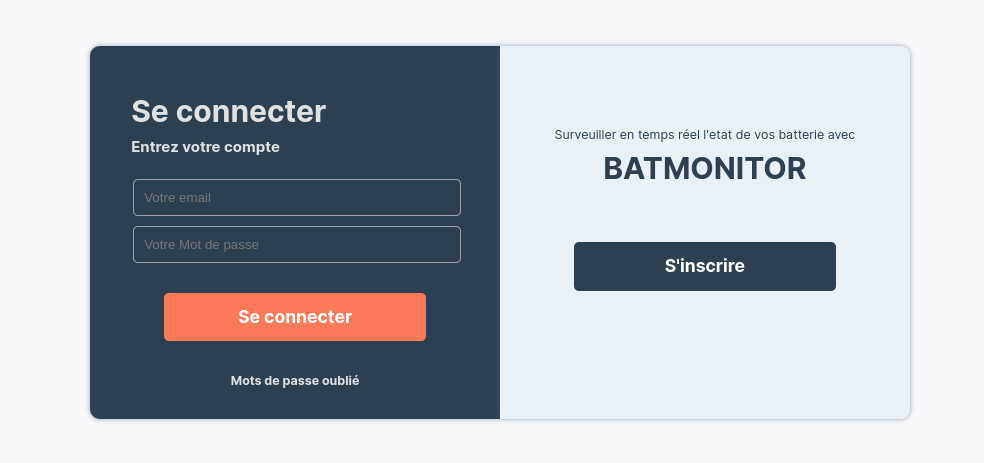
\includegraphics[width=17cm]{./img/interface/login.png}
	\caption{Authentification ( se connecter)}
	\label{fig:relais_5vdc}
\end{figure}

\begin{figure}[H]
	\centering
	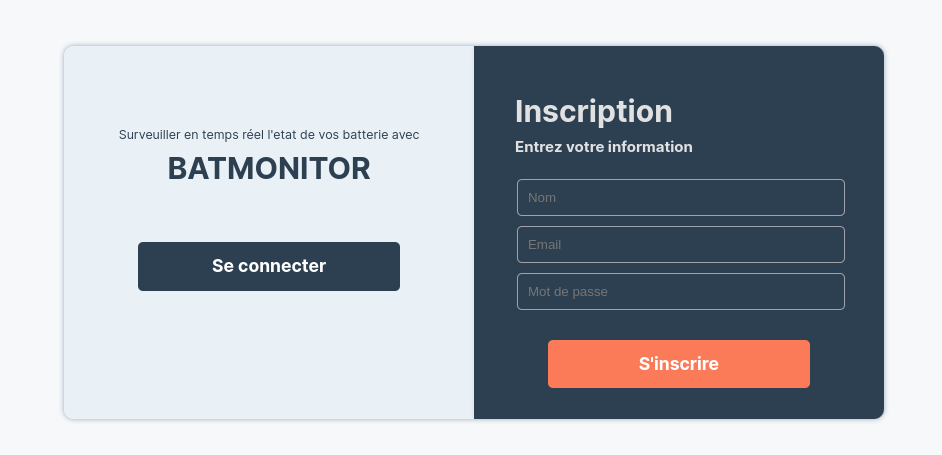
\includegraphics[width=17cm]{./img/interface/singup.png}
	\caption{Authentification (S'inscrire)}
	\label{fig:relais_5vdc}
\end{figure}

\subsection{Page d'accueil}

Cette page permet de visualiser en temps réel les données de chaque batterie, telles que la tension, le courant, la température, ainsi que les graphiques correspondants. Les options de navigation disponibles dépendent du rôle de l'utilisateur. En cliquant sur le bouton \textbf{Détail}, il est possible d'accéder à des informations plus approfondies sur chaque batterie.

\begin{figure}[H]
	\centering
	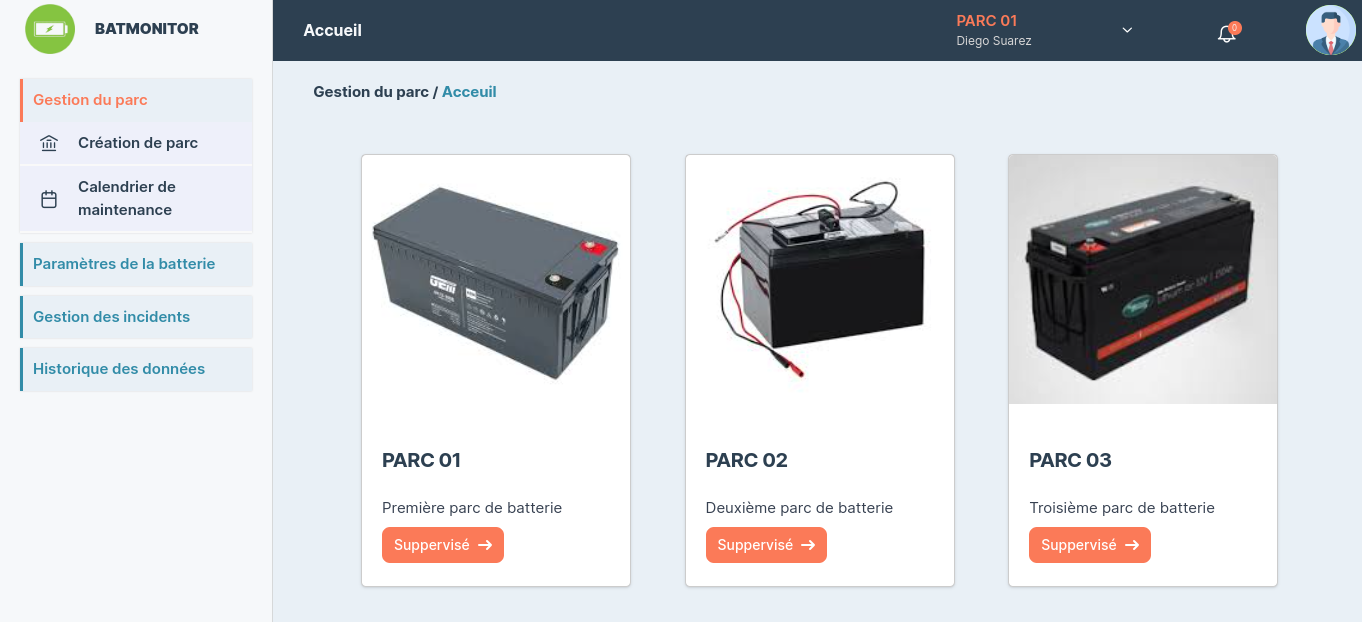
\includegraphics[width=17cm]{./img/Interfaces/acceuil.png}
	\caption{Page d'accueil}
	\label{fig:relais_5vdc}
\end{figure}

\begin{figure}[H]
	\centering
	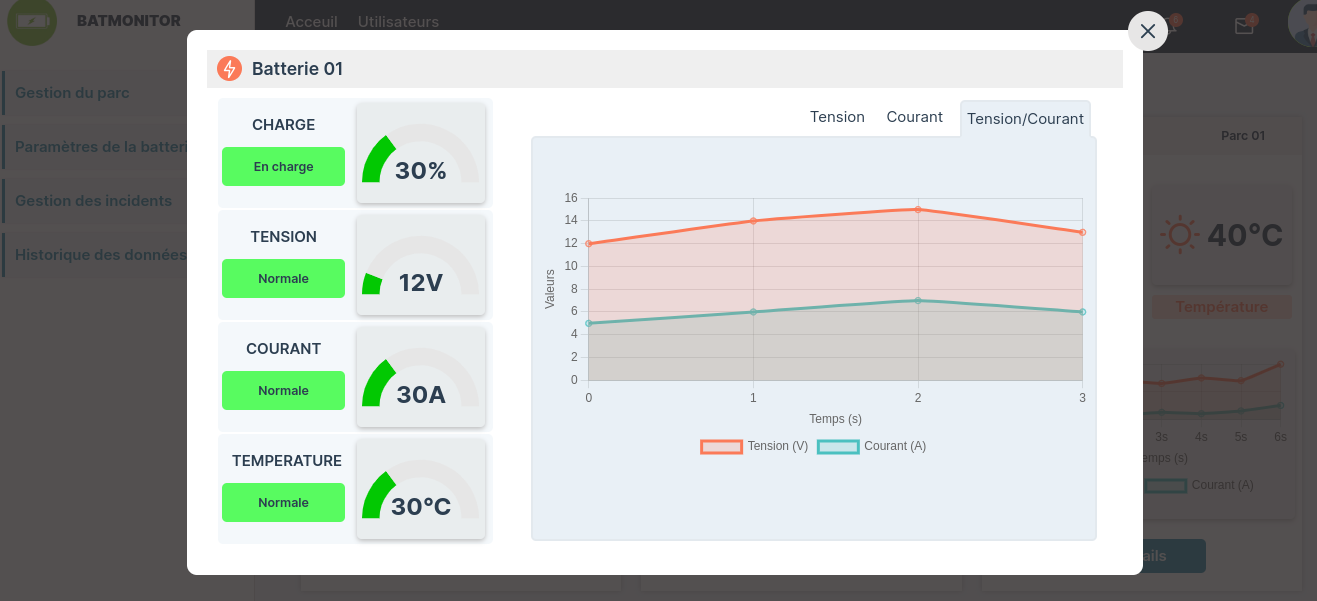
\includegraphics[width=17cm]{./img/interface/detailAcceuil.png}
	\caption{Page détail de batterie}
	\label{fig:relais_5vdc}
\end{figure}

\subsection{Page de gestion du parc}

En accédant à la section \textbf{Gestion du parc} via le menu de navigation, l'utilisateur peut créer un parc, consulter, modifier, visualiser les détails ou supprimer un parc existant. La page dédiée au calendrier de maintenance permet de visualiser les maintenances récentes ainsi que l'historique des interventions. Il est également possible de supprimer ou de modifier la description d'une maintenance.
 
\begin{figure}[H]
	\centering
	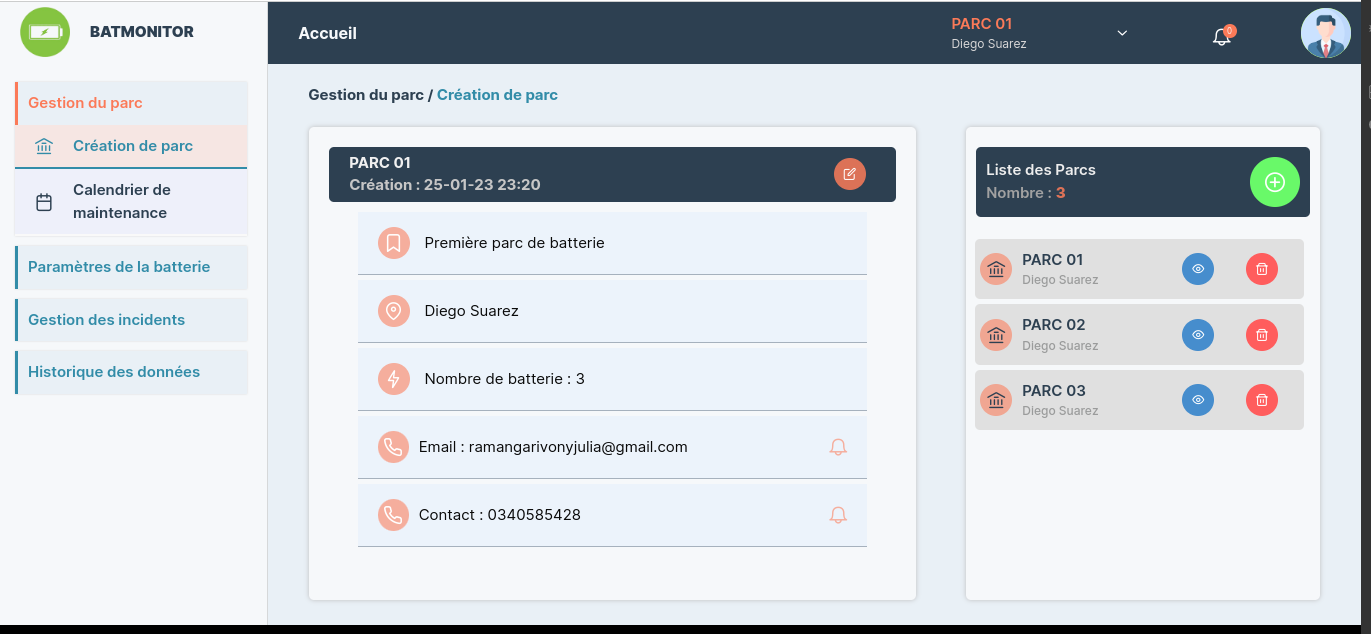
\includegraphics[width=17cm]{./img/Interfaces/gestionParcCreation.png}
	\caption{Gestion de parc sur la création parc}
	\label{fig:relais_5vdc}
\end{figure}


\begin{figure}[H]
	\centering
	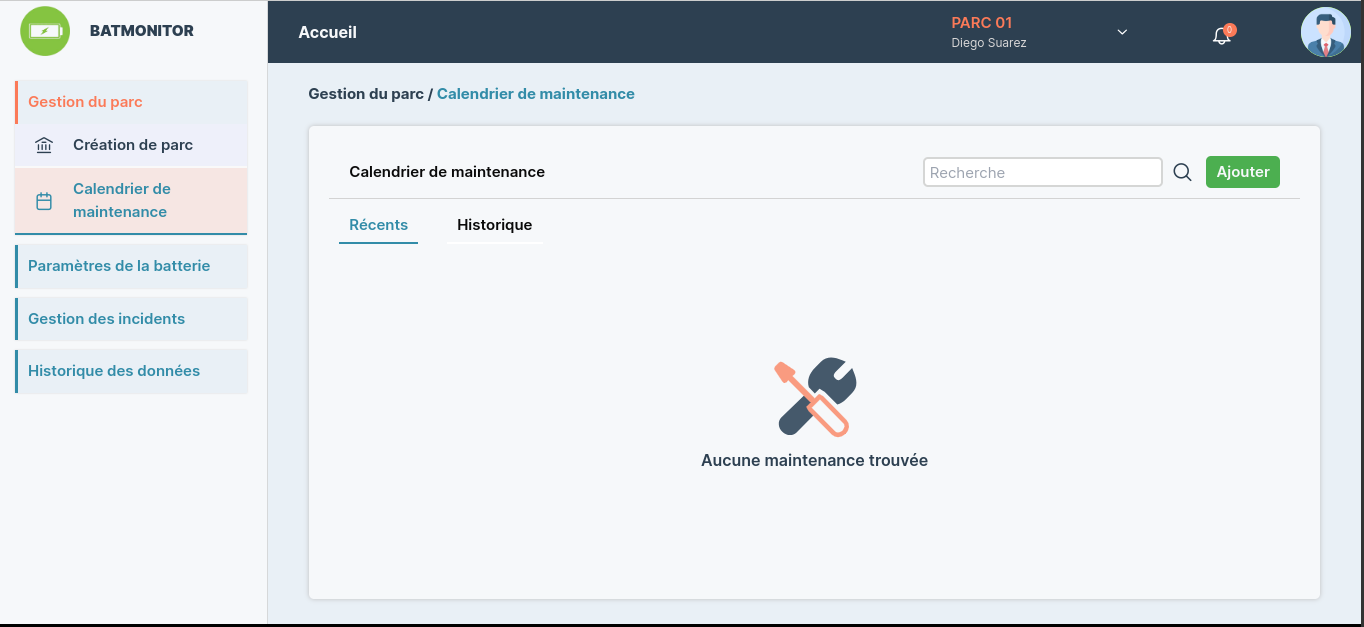
\includegraphics[width=17cm]{./img/Interfaces/gestionParcMaintenance.png}
	\caption{Gestion de parc sur la calendrier de maintenance}
	\label{fig:relais_5vdc}
\end{figure}

\subsection{Paramètres de la batterie}

Cette section permet de consulter les plages de fonctionnement de chaque batterie en affichant tous les paramètres détaillés. En accédant à la section \textbf{Seuils d'alerte}, il est possible de visualiser les seuils de fonctionnement spécifiques à chaque batterie.



\begin{figure}[H]
	\centering
	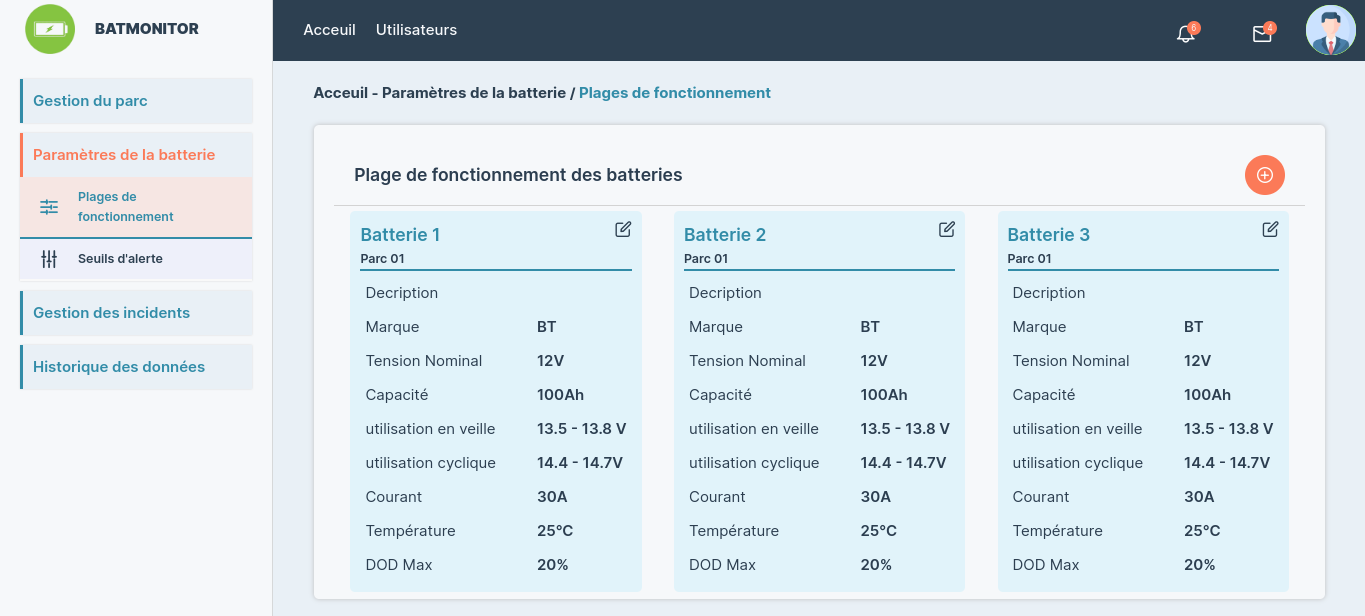
\includegraphics[width=17cm]{./img/interface/PlageFonctionement.png}
	\caption{Paramètres de la batterie sur la plage de fonctionnement}
	\label{fig:relais_5vdc}
\end{figure}

\begin{figure}[H]
	\centering
	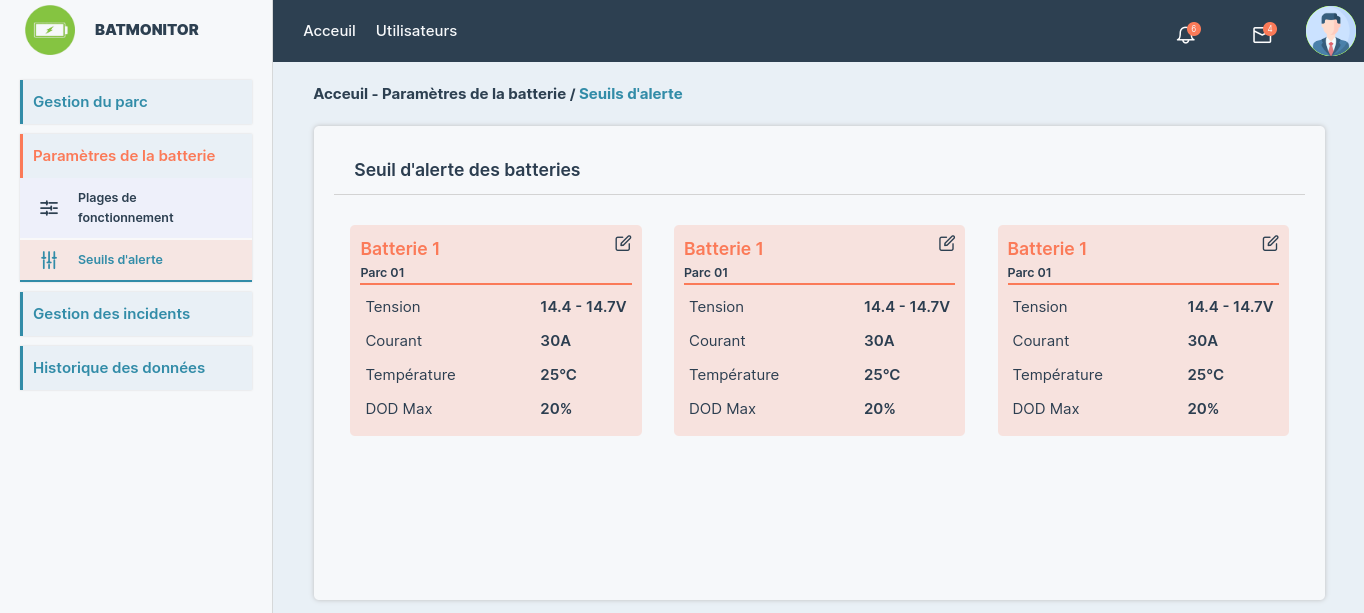
\includegraphics[width=17cm]{./img/interface/seuilAlerte.png}
	\caption{Paramètres de la batterie sur la seuil d'alerte}
	\label{fig:relais_5vdc}
\end{figure}


\subsection{Page de gestion des incidents}

Cette page permet de consulter la liste des incidents récents ainsi que l'historique des incidents. Il est possible d'effectuer une recherche par date via le champ de recherche. En cliquant sur le bouton \textbf{Récent}, les incidents récents s'affichent, tandis que le bouton \textbf{Historique} permet de visualiser les incidents passés.

\begin{figure}[H]
	\centering
	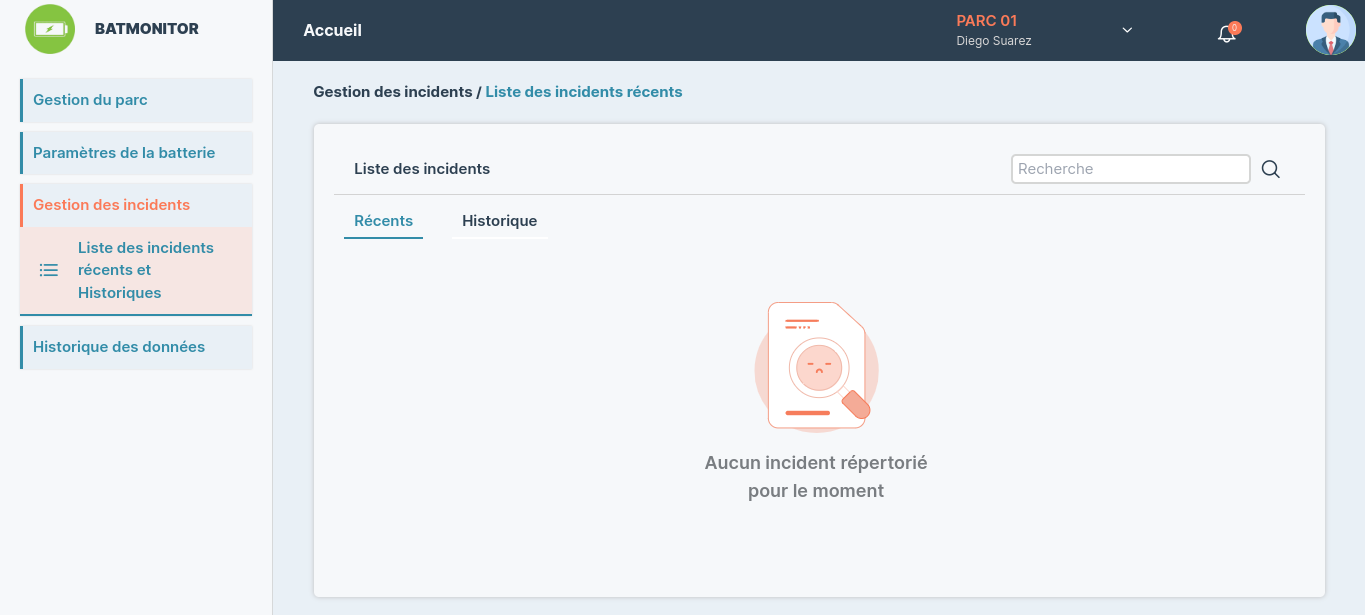
\includegraphics[width=17cm]{./img/interface/listeIncident.png}
	\caption{Page de gestion des incidents sur récent}
	\label{fig:relais_5vdc}
\end{figure}



\subsection{Page d'historique des données}

Cette page permet de visualiser les données stockées sous forme de graphiques, affichant la tension, le courant et la température de chaque batterie en fonction de l'historique des données : jour, semaine, mois ou année.

\begin{figure}[H]
	\centering
	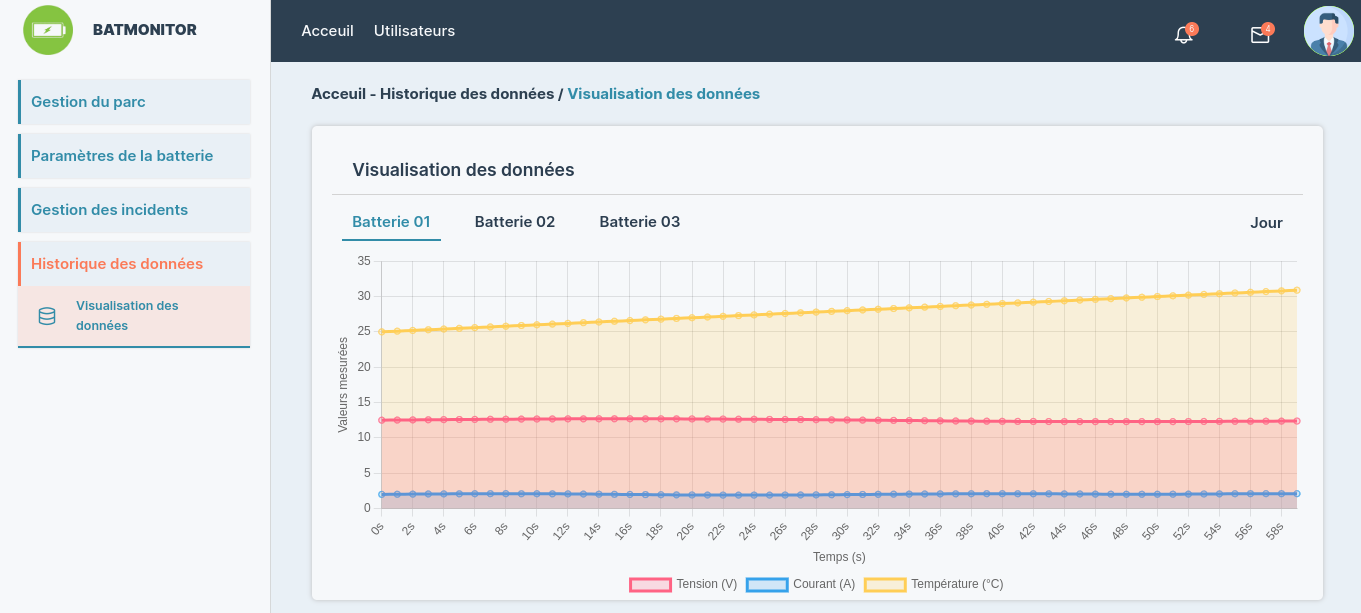
\includegraphics[width=17cm]{./img/interface/visualisationDonne.png}
	\caption{Page d'historique des données}
	\label{fig:relais_5vdc}
\end{figure}

\subsection{Notifications}

En cliquant sur l'icône cloche, l'utilisateur peut accéder aux notifications.

\begin{figure}[H]
	\centering
	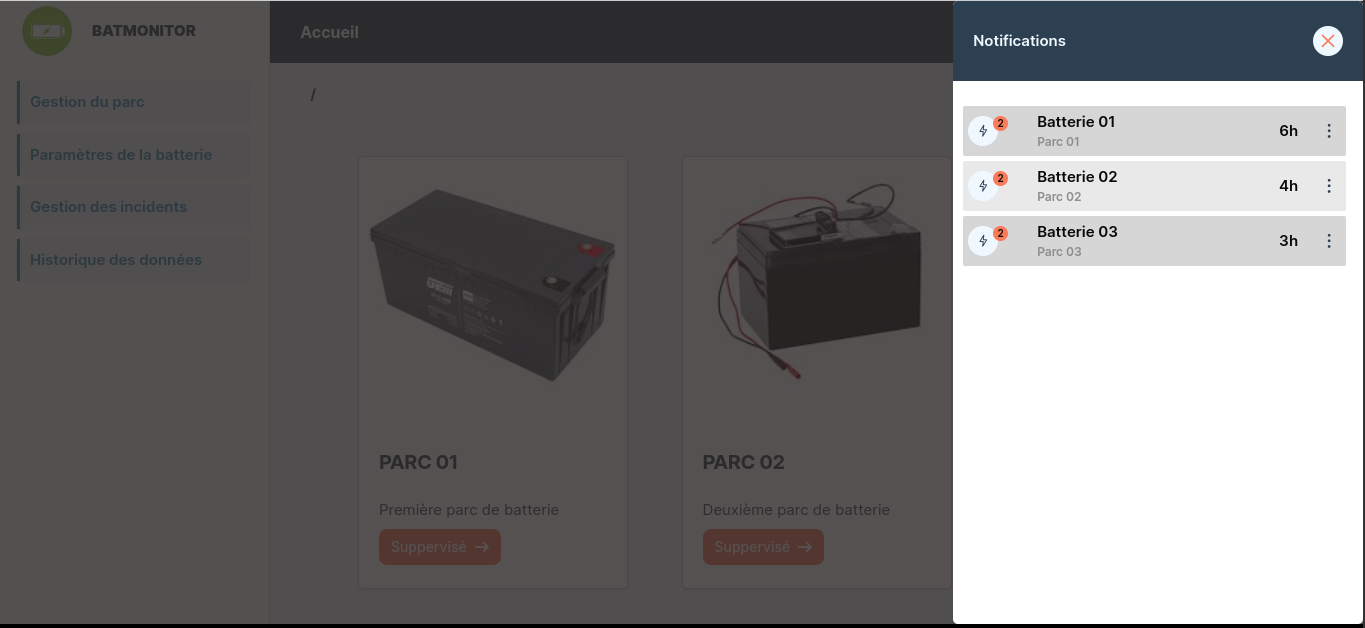
\includegraphics[width=17cm]{./img/interface/notification.png}
	\caption{Notification}
	\label{fig:relais_5vdc}
\end{figure}
\section{Conclusion}

En résumé, le système de gestion et de surveillance développé permet un suivi en temps réel des batteries, offrant une vue d'ensemble précise de leurs paramètres de fonctionnement tels que la tension, le courant et la température. Grâce à l'interface utilisateur intuitive, les utilisateurs peuvent facilement accéder aux informations essentielles, consulter l'historique des données, et gérer les incidents et maintenances avec efficacité. La mise en place des fonctionnalités de notifications et d'alertes assure une réactivité accrue face aux éventuels dysfonctionnements. 


